% coding:utf-8

%----------------------------------------
%FOSAPHY, a LaTeX-Code for a summary of mathematics
%Copyright (C) 2013, Mario Felder, Michael Fallegger

%This program is free software; you can redistribute it and/or
%modify it under the terms of the GNU General Public License
%as published by the Free Software Foundation; either version 2
%of the License, or (at your option) any later version.

%This program is distributed in the hope that it will be useful,
%but WITHOUT ANY WARRANTY; without even the implied warranty of
%MERCHANTABILITY or FITNESS FOR A PARTICULAR PURPOSE.  See the
%GNU General Public License for more details.
%----------------------------------------

\chapter{Repetition}
\section{Kreisgleichung}
Der Mittelpunkt des Kreises wird mit $x_0$ und $y_0$ angegeben.\\
\newline
\[
	\boxed{(x-x_{0})^2+(y-y{0})^2=r^2 }
\]	
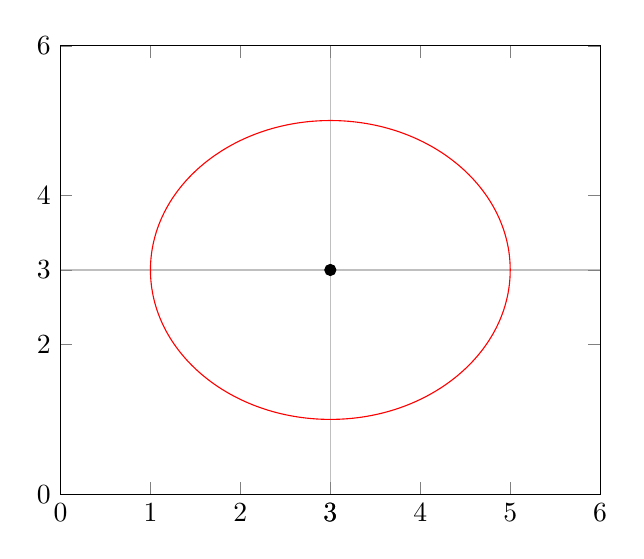
\begin{tikzpicture}
\begin{axis}[
	xmin=0,   xmax=6,
	ymin=0,   ymax=6,
	extra x ticks={3},
	extra y ticks={3},
	extra tick style={grid=major},
]
	\draw[red] \pgfextra{
	  \pgfpathellipse{\pgfplotspointaxisxy{3}{3}}
		{\pgfplotspointaxisdirectionxy{2}{0}}
		{\pgfplotspointaxisdirectionxy{0}{2}}
	  % see also the documentation of 
	  % 'axis direction cs' which
	  % allows a simpler way to draw this ellipse
	};
	\addplot [only marks,mark=*] coordinates { (3,3) };
\end{axis}
\end{tikzpicture}
\\
\\
Rotation um die z-Achse
\[
	\boxed{z=f(x,y)=g(\sqrt{x^2+y^2}}
\]
\\
\\




